\documentclass[12pt,a4paper]{article}

% ---- Packages ----
\usepackage[utf8]{inputenc}
\usepackage[T1]{fontenc}
\usepackage[english]{babel}
\usepackage{geometry}
\geometry{a4paper, margin=2.5cm}

\usepackage{amsmath, amssymb, amsthm}
\usepackage{mathtools}
\usepackage{graphicx}
\usepackage{xcolor}
\usepackage{hyperref}
\usepackage{booktabs}
\usepackage{array}
\usepackage{tabularx}
\usepackage{multirow}
\usepackage{listings}
\usepackage{caption}
\usepackage{subcaption}
\usepackage{float}
\usepackage{enumitem}
\usepackage{csquotes}
\usepackage{setspace}
\usepackage{parskip}
\usepackage{fancyhdr}
\usepackage{titlesec}
\usepackage{microtype}
\usepackage{cite}
\usepackage{algorithm}
\usepackage{algpseudocode}
\usepackage{tikz}
\usetikzlibrary{shapes.geometric, arrows.meta, positioning, fit, backgrounds, calc, decorations.pathreplacing}
\usepackage{pgfplots}
\pgfplotsset{compat=1.18}

% ---- Color definitions ----
\definecolor{darkblue}{RGB}{0,51,102}
\definecolor{medblue}{RGB}{0,102,153}
\definecolor{lightblue}{RGB}{173,216,230}
\definecolor{darkgray}{RGB}{50,50,50}
\definecolor{codegray}{RGB}{245,245,245}
\definecolor{codegreen}{RGB}{0,128,0}
\definecolor{codepurple}{RGB}{128,0,128}
\definecolor{codered}{RGB}{160,0,0}

% ---- Hyperref setup ----
\hypersetup{
    colorlinks=true,
    linkcolor=darkblue,
    citecolor=medblue,
    urlcolor=medblue,
    pdftitle={ROS2 PlanSys and Task Planning: Preliminary Research for DEL-based Multi-Agent Planning},
    pdfauthor={Preliminary Research Document},
}

% ---- Header / Footer ----
\pagestyle{fancy}
\fancyhf{}
\fancyhead[L]{\small\textcolor{darkblue}{\textit{Preliminary Research: DEL-based Task Planning for Multi-Agent Robotics}}}
\fancyhead[R]{\small\thepage}
\fancyfoot[C]{\small\textcolor{darkgray}{\hrule\vspace{2pt}ROS2 | PlanSys2 | EPDDL | Multi-Agent Systems}}
\renewcommand{\headrulewidth}{0.5pt}

% ---- Listings style ----
\lstdefinestyle{ros2style}{
    backgroundcolor=\color{codegray},
    basicstyle=\ttfamily\footnotesize,
    keywordstyle=\color{darkblue}\bfseries,
    commentstyle=\color{codegreen}\itshape,
    stringstyle=\color{codered},
    numberstyle=\tiny\color{darkgray},
    numbers=left,
    breaklines=true,
    breakatwhitespace=false,
    frame=single,
    rulecolor=\color{darkgray},
    tabsize=2,
    captionpos=b,
    showstringspaces=false,
    morekeywords={action, node, launch, package, executor, domain, problem, predicate}
}
\lstset{style=ros2style}

% ---- Theorem environments ----
\theoremstyle{definition}
\newtheorem{definition}{Definition}[section]
\newtheorem{example}{Example}[section]
\theoremstyle{plain}
\newtheorem{proposition}{Proposition}[section]
\newtheorem{remark}{Remark}[section]

\titleformat{\section}{\large\bfseries\color{darkblue}}{\thesection}{1em}{}[\color{medblue}\titlerule]
\titleformat{\subsection}{\normalsize\bfseries\color{darkblue}}{\thesubsection}{1em}{}
\titleformat{\subsubsection}{\normalsize\itshape\color{darkgray}}{\thesubsubsection}{1em}{}

\setlength{\parindent}{0pt}
\setlength{\parskip}{8pt}
\onehalfspacing

\begin{document}

\begin{titlepage}
\begin{center}
\vspace*{1.5cm}

{\color{darkblue}\rule{\linewidth}{1.5pt}}
\vspace{0.5cm}

{\LARGE\bfseries\color{darkblue} ROS2 PlanSys2 and Task Planning for Multiple Robots:\\[0.4em]
\large\color{darkgray} Preliminary Research Toward DEL-based Task Planning\\
with EPDDL for Multi-Agent Robotics in Uncertain Environments}

\vspace{0.5cm}
{\color{darkblue}\rule{\linewidth}{1.5pt}}

\vspace{1.5cm}

{\large Preliminary Research Document}\\[0.5em]
{\normalsize Preliminary research in the context of epistemic multi-agent planning,\\
grounded in Dynamic Epistemic Logic and the EPDDL framework}

\vspace{2cm}

\begin{tabular}{rl}
\textbf{Research Area:} & Autonomous Robotics \& Epistemic Planning \\
\textbf{Keywords:}      & ROS2, PlanSys2, PDDL, DEL, EPDDL, Multi-Robot Systems \\
\textbf{Document Type:} & Preliminary Research / State of the Art \\
\textbf{Version:}       & 1.0 \\
\end{tabular}

\vspace{3cm}

{\color{darkgray}\textit{Haniel Ulises}}

\vfill
{\small\color{darkgray} This document is a preliminary academic survey compiled in preparation for research on DEL-based epistemic task planning using EPDDL for multi-agent robotic systems operating under partial observability. It is not a finished publication.}
\end{center}
\end{titlepage}

\newpage
\begin{abstract}
\noindent
The increasing deployment of autonomous robotic systems in complex, uncertain, and partially observable environments demands planning formalisms that transcend the capabilities of classical automated planning. This document constitutes a preliminary research survey covering two major pillars of the target research agenda: (i)~the state of the art in robot task planning using the Robot Operating System 2 (ROS2), with particular focus on the PlanSys2 framework and its PDDL-based planning infrastructure; and (ii)~the theoretical and conceptual foundations of Dynamic Epistemic Logic (DEL) and the Epistemic Planning Domain Definition Language (EPDDL), as introduced by Burigana and Fabiano for IPC 2026. The ultimate motivation of this survey is to chart a research path toward a DEL-based multi-agent task planning system for heterogeneous robot fleets operating under epistemic uncertainty. We discuss the architecture of ROS2 multi-robot systems, the structure and limitations of existing PDDL-based planners in robotics, the semantics of epistemic states and actions in DEL, and the syntactic mechanisms of EPDDL. We conclude with an analysis of the integration challenges and open research questions at the intersection of these fields.
\end{abstract}

\vspace{1em}
\noindent\textbf{Keywords:} ROS2, PlanSys2, PDDL, task planning, multi-robot systems, Dynamic Epistemic Logic, epistemic planning, EPDDL, partial observability, multi-agent systems.

\newpage
\tableofcontents

\newpage
\section{Introduction}
\label{sec:intro}

Modern autonomous robotic systems are increasingly expected to operate in environments that are shared with other agents---whether human operators, other autonomous robots, or dynamically changing physical conditions---where the state of the world is not fully and reliably observable. A warehouse robot fleet, a team of search-and-rescue drones, or a collaborative assembly line all require their constituent agents to reason not only about what is true in the world, but also about what each agent \textit{knows}, what each agent \textit{believes}, and what each agent knows or believes about the epistemic states of others. Classical task planning formalisms, such as PDDL (Planning Domain Definition Language), remain the de facto standard in practical robotic systems and are supported by major middleware frameworks such as ROS2 through tools like PlanSys2. However, classical planning fundamentally assumes a fully observable, deterministic environment and a single omniscient planning agent---assumptions that are routinely violated in realistic multi-robot deployments.

The objective of this document is to establish a comprehensive preliminary understanding of two converging research areas: the engineering and middleware infrastructure for task planning in ROS2 multi-robot systems, and the theoretical framework provided by Dynamic Epistemic Logic (DEL) and its associated language, EPDDL, for epistemic multi-agent planning. Together, these two pillars form the foundation upon which a future system can be built: one capable of reasoning about the knowledge and beliefs of individual robots, performing multi-agent coordination under partial observability, and expressing rich epistemic goals such as ``robot $A$ knows whether corridor $c$ is blocked,'' or ``it is common knowledge among all robots that the package has been delivered.''

Section~\ref{sec:ros2} introduces ROS2 as a middleware architecture, covering its communication model, multi-robot support, and lifecycle management. Section~\ref{sec:plansys2} examines PlanSys2, the primary task planning framework for ROS2, including its PDDL integration, executor architecture, and known limitations. Section~\ref{sec:multirobot} surveys the state of the art in multi-robot coordination and planning within ROS2. Section~\ref{sec:del} provides an accessible but technically grounded introduction to Dynamic Epistemic Logic, covering epistemic states, epistemic actions, and the product update semantics. Section~\ref{sec:epddl} presents EPDDL, the Epistemic Planning Domain Definition Language, describing its syntax, action type libraries, and relationship to existing DEL fragments. Section~\ref{sec:integration} analyzes the integration challenges and proposes a conceptual architecture for a DEL-based ROS2 planning system. Section~\ref{sec:conclusion} summarizes the findings and outlines open research questions.

\newpage
\section{ROS2: Architecture and Multi-Robot Infrastructure}
\label{sec:ros2}

\subsection{Overview and Design Principles}

The Robot Operating System 2 (ROS2) is an open-source middleware framework designed to provide a flexible and modular infrastructure for robotic software development~\cite{macenski2022robot}. Unlike its predecessor ROS1, which relied on a centralized master node and a single-process communication model, ROS2 is built atop the Data Distribution Service (DDS) standard, providing a fully decentralized, quality-of-service-aware publish-subscribe communication layer. This architectural shift makes ROS2 fundamentally more suited to multi-robot deployments, real-time systems, and industrial applications.

The core communication abstractions in ROS2 are \textit{nodes}, \textit{topics}, \textit{services}, and \textit{actions}. A node is the fundamental computational unit---a process encapsulating a specific functional capability. Topics implement an asynchronous, many-to-many publish-subscribe pattern. Services implement synchronous request-reply communication. Actions, which are particularly important for task planning integration, extend services with long-running asynchronous goals, feedback during execution, and cancellation semantics.

\begin{figure}[H]
\centering
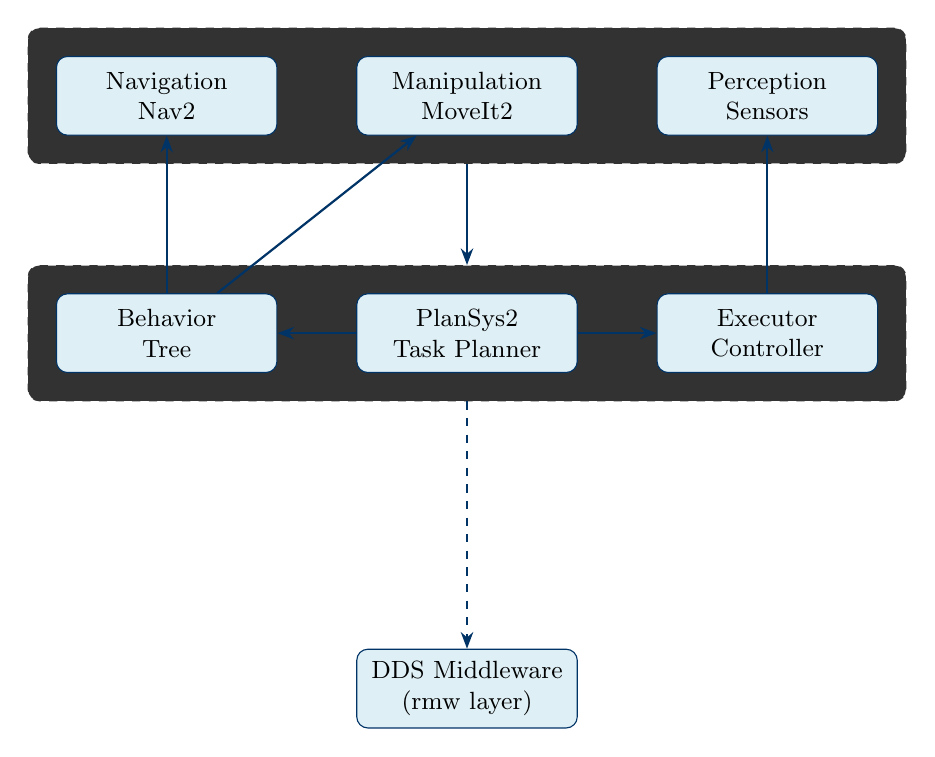
\begin{tikzpicture}[
    node distance=1.5cm,
    block/.style={rectangle, draw=darkblue, fill=lightblue!40, rounded corners, minimum width=2.8cm, minimum height=1cm, font=\small, align=center},
    layer/.style={rectangle, draw=medblue, dashed, fill=blue!5, rounded corners, inner sep=10pt},
    arrow/.style={-{Stealth[length=6pt]}, thick, color=darkblue},
    label/.style={font=\small\itshape, color=darkgray}
]
\node[block] (nav) {Navigation\\Nav2};
\node[block, right=1cm of nav] (manip) {Manipulation\\MoveIt2};
\node[block, right=1cm of manip] (perc) {Perception\\Sensors};
\node[block, below=2cm of manip] (plan) {PlanSys2\\Task Planner};
\node[block, below=2cm of nav] (bt) {Behavior\\Tree};
\node[block, below=2cm of perc] (exec) {Executor\\Controller};
\node[block, below=3.5cm of plan] (dds) {DDS Middleware\\(rmw layer)};

\begin{scope}[on background layer]
\node[layer, fit=(nav)(manip)(perc), label=above:{\textbf{Application Layer}}] (applayer) {};
\node[layer, fit=(plan)(bt)(exec), label=above:{\textbf{Planning \& Control Layer}}] (planlayer) {};
\end{scope}

\draw[arrow] (plan) -- (bt);
\draw[arrow] (bt) -- (nav);
\draw[arrow] (bt) -- (manip);
\draw[arrow] (exec) -- (perc);
\draw[arrow] (plan) -- (exec);
\draw[arrow] (applayer.south) -- (planlayer.north);
\draw[arrow, dashed] (planlayer.south) -- (dds.north);
\end{tikzpicture}
\caption{Simplified layered architecture of a ROS2 robot system. The task planner (PlanSys2) operates within the Planning \& Control Layer, interfacing with navigation, manipulation, and perception via behavior trees and action servers, all underpinned by DDS.}
\label{fig:ros2arch}
\end{figure}

\subsection{DDS and the Communication Model}

The choice of DDS as the underlying transport mechanism for ROS2 has deep implications for multi-robot deployments. DDS implements a data-centric publish-subscribe (DCPS) model where data flows between publishers and subscribers through a shared data space---the \textit{Global Data Space}---without the need for a centralized broker. Each DDS participant declares its intent to publish or subscribe to a given \textit{Topic}, identified by name and data type. Quality of Service (QoS) policies govern reliability (reliable vs.\ best-effort), durability (transient local vs.\ volatile), deadline, and liveliness.

For multi-robot systems, DDS offers native support for distributed discovery: robots on the same network segment automatically discover each other's nodes, topics, and services without manual configuration. This is mediated through the \textit{DDS Domain} abstraction, which partitions the shared data space into independent communication contexts. Different robot fleets or subsystems can be assigned different domain IDs to prevent cross-contamination of messages.

\subsection{Node Lifecycle and Managed Nodes}

ROS2 introduced a formal node lifecycle management protocol, defining a set of states (Unconfigured, Inactive, Active, Finalized) and transitions between them. Managed nodes follow this lifecycle, enabling orchestrated startup, shutdown, and error recovery sequences. From a task planning perspective, the lifecycle model provides a principled mechanism for activating and deactivating capabilities on demand---for example, a planning system may activate a navigation capability only when an action requiring navigation is dispatched.

\subsection{Multi-Robot Namespacing and Coordination}

ROS2 addresses the multi-robot naming problem through a hierarchical namespace mechanism. Each robot is typically assigned a unique namespace prefix (e.g., \texttt{/robot1}, \texttt{/robot2}), and all its nodes, topics, services, and actions are scoped under that prefix. This simple convention allows multiple robot instances to coexist on the same DDS domain without topic collisions, and enables a centralized planning or coordination node to address individual robots by namespace.

However, namespacing alone is insufficient for true multi-robot coordination. Coordination requires shared state representation, inter-robot communication protocols, conflict resolution, and synchronized action dispatch---all of which must be built on top of the raw namespace infrastructure. Several frameworks and design patterns have emerged to address these needs, as discussed in Section~\ref{sec:multirobot}.

\subsection{ROS2 Actions and Task Execution}

The ROS2 action protocol is the primary mechanism for integrating task planning with robot execution. An action server exposes a goal interface, accepting goal requests from action clients, providing periodic feedback, and returning a final result. This maps directly to the classical planning loop: the planner emits a sequence of actions, each dispatched as a goal to the corresponding action server, and execution proceeds with feedback monitored by the planner or a behavior executive.

The standard action message types in ROS2 are defined using the \texttt{.action} interface format, which concatenates a goal, result, and feedback message definition. The interface is implemented over the service protocol with asynchronous semantics, providing automatic state management (ACCEPTED, EXECUTING, CANCELING, SUCCEEDED, ABORTED, CANCELED) accessible to both the client and the server.

\newpage
\section{PlanSys2: Task Planning in ROS2}
\label{sec:plansys2}

\subsection{Architecture Overview}

PlanSys2 is the primary open-source framework for PDDL-based task planning in ROS2~\cite{martin2021plansys2}. It provides a modular, multi-node architecture that integrates domain and problem management, plan generation via external PDDL solvers, and plan execution via a behavior-tree-based action dispatcher. Figure~\ref{fig:plansys2arch} illustrates the internal architecture of PlanSys2.

\begin{figure}[H]
\centering
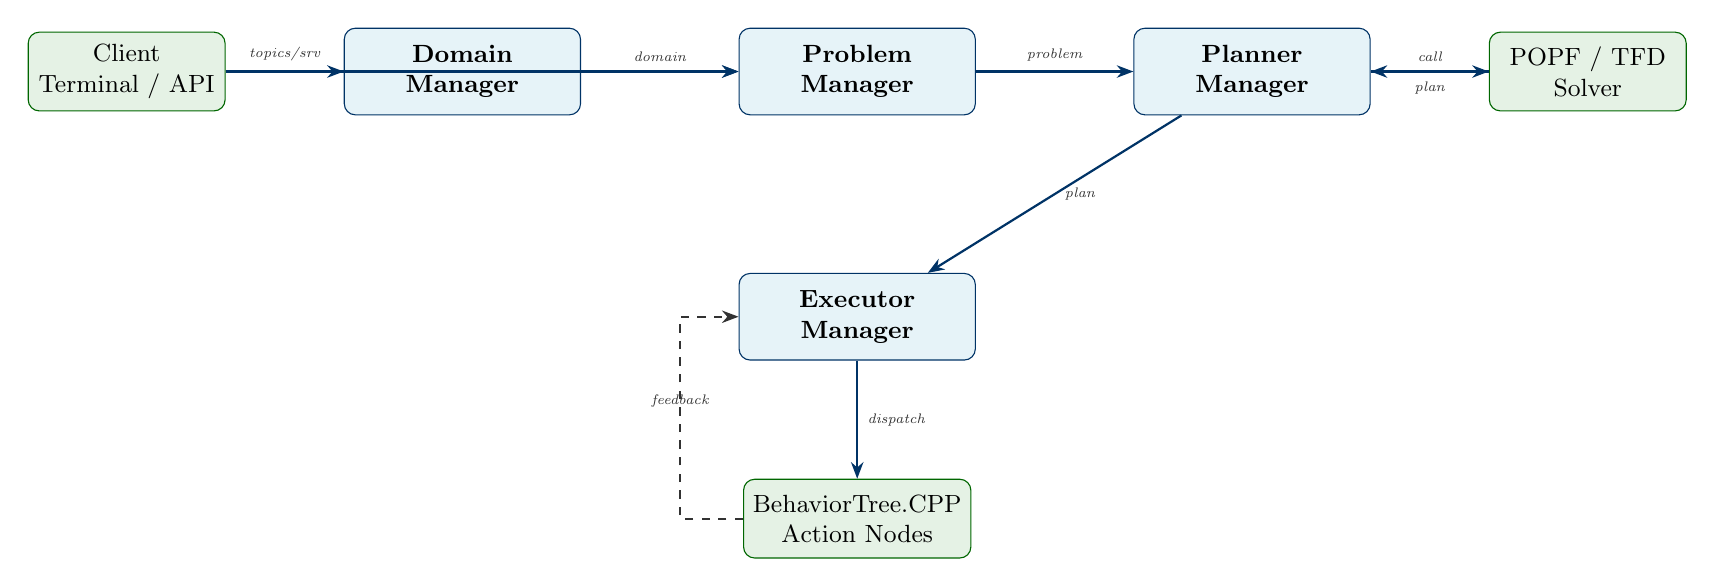
\begin{tikzpicture}[
    box/.style={rectangle, draw=darkblue, fill=lightblue!30, rounded corners=4pt, minimum width=3cm, minimum height=1.1cm, font=\small\bfseries, align=center},
    ext/.style={rectangle, draw=codegreen!80!black, fill=codegreen!10, rounded corners=4pt, minimum width=2.5cm, minimum height=1cm, font=\small, align=center},
    arr/.style={-{Stealth[length=6pt]}, thick, darkblue},
    darr/.style={-{Stealth[length=6pt]}, thick, darkgray, dashed},
    lbl/.style={font=\tiny\itshape, darkgray}
]

\node[box] (dm) {Domain\\Manager};
\node[box, right=2cm of dm] (pm) {Problem\\Manager};
\node[box, right=2cm of pm] (pl) {Planner\\Manager};
\node[box, below=2cm of pm] (ex) {Executor\\Manager};
\node[ext, left=1.5cm of dm] (client) {Client\\Terminal / API};
\node[ext, right=1.5cm of pl] (solver) {POPF / TFD\\Solver};
\node[ext, below=1.5cm of ex] (bt) {BehaviorTree.CPP\\Action Nodes};

\draw[arr] (client) -- (dm) node[midway, above, lbl]{topics/srv};
\draw[arr] (client) -- (pm);
\draw[arr] (dm) -- (pm) node[midway, above, lbl]{domain};
\draw[arr] (pm) -- (pl) node[midway, above, lbl]{problem};
\draw[arr] (pl) -- (solver) node[midway, above, lbl]{call};
\draw[arr] (solver) -- (pl) node[midway, below, lbl]{plan};
\draw[arr] (pl) -- (ex) node[midway, right, lbl]{plan};
\draw[arr] (ex) -- (bt) node[midway, right, lbl]{dispatch};
\draw[darr] (bt.west) -- ++(-0.8,0) |- (ex.west) node[near start, above, lbl]{feedback};
\end{tikzpicture}
\caption{Internal architecture of PlanSys2. The Domain Manager, Problem Manager, Planner Manager, and Executor Manager are separate ROS2 nodes communicating over topics and services. An external solver (e.g., POPF or TFD) is called by the Planner Manager. The Executor dispatches actions to BehaviorTree.CPP action nodes.}
\label{fig:plansys2arch}
\end{figure}

PlanSys2 decouples the responsibilities of domain management, problem management, planning, and execution into separate ROS2 nodes, following the microservice design principle. This separation allows each component to be independently replaced, updated, or scaled.

\subsection{Domain and Problem Management}

The Domain Manager maintains the PDDL domain specification for the planning problem. It receives predicate updates and type definitions and exposes them to the Planner Manager on demand. The Problem Manager maintains the dynamic planning problem---the current set of predicates (the world state), the set of instantiated objects, and the current goal specification. It is the primary interface through which the robot system updates its internal world model as perception events are received.

The interface to both managers is exposed as a set of ROS2 services and topics, allowing any node in the system to add or remove predicates, add or remove objects, and update the goal. PlanSys2 also provides a terminal client that allows a human operator to interact with the system through a command-line interface.

\subsection{Plan Generation and PDDL Solvers}

PlanSys2 delegates the actual planning computation to external PDDL planners, interfacing with them through a plugin architecture. The most commonly used solvers are POPF (Partial Order Planning Forward-chaining)~\cite{coles2010forward} and TFD (Temporal Fast Downward), both of which support temporal PDDL with durative actions. PlanSys2 extends standard PDDL with a set of custom predicates and action types that map to ROS2 action servers, enabling the planner to reason about actions that have temporal extents and concurrent execution.

The planning loop in PlanSys2 is triggered by a goal update or a world state change that renders the current plan invalid. The system then serializes the current domain and problem, calls the solver, receives the plan, and passes it to the Executor Manager.

\subsection{Execution via Behavior Trees}

Plan execution in PlanSys2 is mediated by the BehaviorTree.CPP library~\cite{faconti2018behaviortree}. Each action in the PDDL domain is associated with a behavior tree node that implements the action's execution logic, including pre-condition verification, execution, and post-condition assertion. The Executor Manager constructs a behavior tree from the plan sequence and runs it, monitoring each action for success, failure, or timeout.

The use of behavior trees for execution provides a structured approach to failure recovery: individual tree nodes can implement retry logic, fallback behaviors, and conditional execution. However, the behavior tree is constructed statically from the plan, and replanning must be explicitly triggered when execution deviates from expectations.

\subsection{Known Limitations of PlanSys2}

Despite its practical utility, PlanSys2 exhibits a number of limitations that are directly relevant to the goals of this research:

\textbf{Epistemic limitations.} The PDDL model underlying PlanSys2 is fundamentally a classical single-agent planning model. The world state is represented as a set of ground predicates that is assumed to be fully known to the planner. There is no representation of what individual agents know or believe, no mechanism for expressing epistemic goals, and no support for actions that change the knowledge state of an agent without changing the physical world.

\textbf{Partial observability.} PlanSys2 does not natively handle partial observability. Sensor uncertainty, missing observations, and conflicting percepts must be handled at the perception layer, outside the planner, before updating the problem's predicate set. The planner always assumes that the predicates it receives reflect the true world state.

\textbf{Multi-agent coordination.} PlanSys2 is designed for single-robot planning with external action servers. While multiple PlanSys2 instances can run simultaneously---one per robot---there is no native mechanism for cross-robot plan coordination, shared world state representation, or multi-agent goal management.

\textbf{Solver expressivity.} The solvers supported by PlanSys2 (POPF, TFD) implement classical or temporal planning with no support for epistemic or probabilistic reasoning. Extending PlanSys2 to use an epistemic planner would require a new solver plugin and potentially a restructured problem representation.

These limitations motivate the core research objective: to develop a framework that integrates the engineering infrastructure of ROS2 and PlanSys2 with the expressive semantics of DEL-based epistemic planning.

% =========================================================
\newpage
\section{Multi-Robot Systems in ROS2}
\label{sec:multirobot}
% =========================================================

\subsection{Architectural Patterns for Multi-Robot Systems}

Multi-robot systems in ROS2 are typically organized according to one of three architectural patterns: \textit{centralized}, \textit{decentralized}, or \textit{hierarchical}. In a centralized architecture, a single master node maintains a global world model and generates plans for all robots; robots execute actions and report results back. This architecture is straightforward to implement and guarantees global consistency, but introduces a single point of failure and does not scale well with fleet size. In a decentralized architecture, each robot operates as an independent planning agent, communicating with peers to resolve conflicts and share observations. This is more fault-tolerant but requires sophisticated consensus and coordination protocols. A hierarchical architecture---which is arguably the most practically relevant for the target research---combines a fleet-level planner with robot-level planners, where the fleet planner decomposes high-level goals into sub-goals assigned to individual robots, and each robot executes its sub-plan locally.

\subsection{Multi-Robot Navigation and Coordination}

Navigation in multi-robot ROS2 systems is typically managed by the Nav2 stack, which provides autonomous navigation, path planning, and obstacle avoidance for individual robots. Nav2 supports namespaced multi-robot deployments, where each robot instance runs its own Nav2 stack under its namespace. Coordination between robots for conflict-free navigation requires additional components, typically implemented as a fleet management layer that allocates navigation goals and resolves spatial conflicts.

The \texttt{nav2\_bringup} package provides launch configurations for multi-robot scenarios, and community packages such as \texttt{nav2\_fleet} and \texttt{fleet\_adapter} (developed in the context of the Open-RMF framework) provide higher-level fleet management. Open-RMF (Open Robotics Middleware Framework) is of particular interest as it provides a standardized interface for multi-fleet, multi-robot task allocation and coordination in shared environments~\cite{openrmf2021}.

\subsection{Task Allocation and Multi-Agent Planning}

Task allocation in multi-robot systems is the problem of assigning tasks to robots so as to optimize some objective (e.g., minimize makespan, maximize coverage, balance load) subject to robot capabilities and resource constraints. Classical approaches include market-based auction methods (e.g., CBBA, MRTA), integer programming formulations, and heuristic search algorithms. More recently, multi-agent planning approaches have been explored, where the task allocation problem is formulated as a multi-agent planning problem and solved by a dedicated planner.

In the context of ROS2 and PlanSys2, several research efforts have proposed extensions to support multi-robot scenarios. One notable approach is to run a single PlanSys2 instance with multiple robot agents modeled as PDDL objects, and to generate plans that explicitly assign actions to robots. This approach leverages standard multi-agent PDDL (MA-PDDL) or MASTRIPS extensions to express agent-specific actions and shared resources. However, such approaches remain within the classical planning paradigm and inherit all its epistemic limitations.

\subsection{Shared World Modeling}

A fundamental challenge in multi-robot systems is maintaining a shared, consistent world model across all agents. Each robot has its own partial view of the world derived from its local sensors, and these views must be fused into a global representation that the planner can reason over. In ROS2 systems, this is typically addressed through shared semantic maps or blackboard-style data structures accessible to all nodes.

From an epistemic planning perspective, the problem of shared world modeling is more subtle: it is not always desirable---or possible---to maintain a single globally consistent world model. Different robots may have genuinely different beliefs about the state of the world, and those differences are themselves semantically meaningful. An epistemic planner must be able to represent and reason about these individual perspectives, plan actions that resolve epistemic differences (e.g., one robot sharing its observation with another), and formulate goals that refer explicitly to the knowledge states of individual robots.

\begin{figure}[H]
\centering
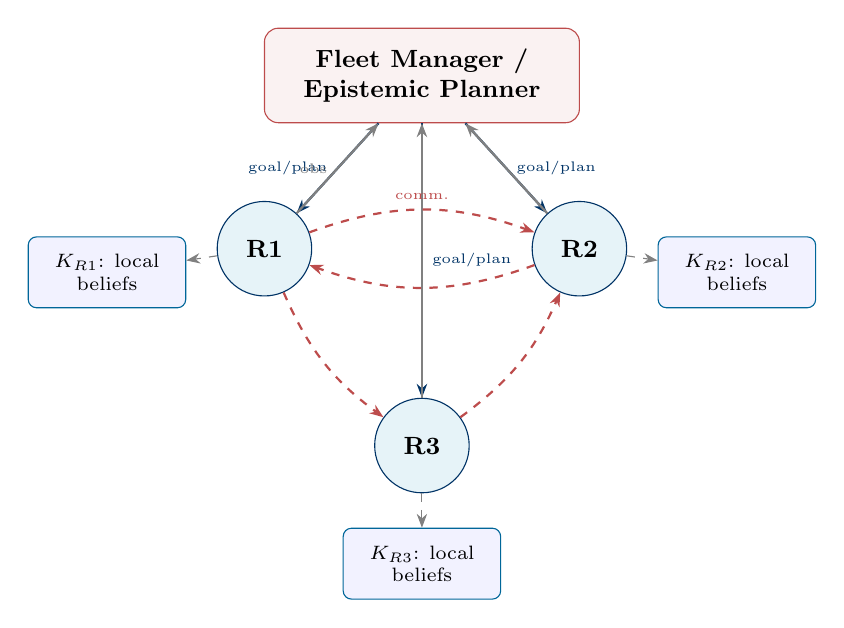
\begin{tikzpicture}[
    robot/.style={circle, draw=darkblue, fill=lightblue!30, minimum size=1.2cm, font=\small\bfseries},
    kb/.style={rectangle, draw=medblue, fill=blue!5, rounded corners=3pt, minimum width=2cm, minimum height=0.9cm, font=\scriptsize, align=center},
    fleet/.style={rectangle, draw=codered!70, fill=codered!5, rounded corners=5pt, minimum width=4cm, minimum height=1.2cm, font=\small\bfseries, align=center},
    arr/.style={-{Stealth[length=5pt]}, thick},
    obs/.style={-{Stealth[length=5pt]}, dashed, gray}
]

\node[robot] (r1) at (0,0) {R1};
\node[robot] (r2) at (4,0) {R2};
\node[robot] (r3) at (2,-2.5) {R3};
\node[fleet] (fm) at (2,2.2) {Fleet Manager /\\Epistemic Planner};
\node[kb] (kb1) at (-2,-0.3) {$K_{R1}$: local\\beliefs};
\node[kb] (kb2) at (6,-0.3) {$K_{R2}$: local\\beliefs};
\node[kb] (kb3) at (2,-4) {$K_{R3}$: local\\beliefs};

\draw[arr, darkblue] (fm) -- (r1) node[midway, left, font=\tiny]{goal/plan};
\draw[arr, darkblue] (fm) -- (r2) node[midway, right, font=\tiny]{goal/plan};
\draw[arr, darkblue] (fm) -- (r3) node[midway, right, font=\tiny]{goal/plan};
\draw[arr, gray] (r1) -- (fm) node[midway, left, font=\tiny]{obs};
\draw[arr, gray] (r2) -- (fm);
\draw[arr, gray] (r3) -- (fm);

\draw[obs] (r1) -- (kb1);
\draw[obs] (r2) -- (kb2);
\draw[obs] (r3) -- (kb3);

\draw[arr, dashed, codered!70] (r1) to[bend left=20] node[midway, above, font=\tiny]{comm.} (r2);
\draw[arr, dashed, codered!70] (r2) to[bend left=20] (r1);
\draw[arr, dashed, codered!70] (r1) to[bend right=15] (r3);
\draw[arr, dashed, codered!70] (r3) to[bend right=15] (r2);
\end{tikzpicture}
\caption{Multi-robot system architecture with a fleet-level epistemic planner and robot-level local knowledge bases. Robots communicate observations to the fleet planner and can also engage in peer-to-peer communication, giving rise to heterogeneous epistemic states.}
\label{fig:multirobot}
\end{figure}

\newpage
\section{Dynamic Epistemic Logic: Foundations for Epistemic Planning}
\label{sec:del}

\subsection{Motivation: From Classical to Epistemic Planning}

Classical planning, as formalized in STRIPS and PDDL, operates over a deterministic, fully observable world. The state of the world is a complete assignment of truth values to a finite set of propositional atoms, and actions transform states deterministically. This model is well-understood and computationally tractable in restricted fragments, but it cannot represent---let alone reason about---the knowledge states of individual agents, uncertainty about the current state of the world, or the epistemic effects of communication actions.

Dynamic Epistemic Logic (DEL)~\cite{baltag1998logic, vanditmarsch2007} provides a rigorous formal framework for reasoning about knowledge, belief, and informational change in multi-agent systems. At its core, DEL extends classical propositional logic with \textit{modal operators} that allow one to express statements such as ``agent $i$ knows that $\varphi$,'' ``agent $i$ believes that agent $j$ does not know whether $p$,'' or ``it is common knowledge among all agents that $\varphi$,'' and provides a formal semantics for how these truth values change when epistemic actions (announcements, observations, deceptions) are applied.

\subsection{Epistemic States and Kripke Semantics}

The semantic foundation of DEL is the \textit{Kripke model}, which represents an agent's epistemic state as a set of possible worlds together with accessibility relations.

\begin{definition}[Multi-Agent Epistemic Model]
A multi-agent epistemic model is a triple $M = (W, R, L)$ where:
\begin{itemize}[noitemsep]
\item $W \neq \emptyset$ is a finite set of \textit{possible worlds};
\item $R : \mathrm{Ag} \to 2^{W \times W}$ assigns to each agent $i \in \mathrm{Ag}$ an \textit{accessibility relation} $R_i \subseteq W \times W$; and
\item $L : W \to 2^P$ assigns to each world a \textit{label}---the set of propositional atoms true in that world.
\end{itemize}
An epistemic state is a pair $s = (M, W_d)$ where $W_d \subseteq W$ is a non-empty set of \textit{designated worlds}.
\end{definition}

Intuitively, each world represents a possible configuration of the physical environment. The accessibility relation $w R_i v$ means that in world $w$, agent $i$ considers world $v$ to be a possibility consistent with its current observations. The designated worlds represent the worlds that are genuinely possible given what is actually known.

The truth of epistemic formulas is defined recursively. A formula $\Box_i \varphi$ (``agent $i$ knows/believes $\varphi$'') holds in a world $w$ of model $M$ if and only if $\varphi$ holds in all worlds $v$ accessible from $w$ via $R_i$:
\[
(M, w) \models \Box_i \varphi \iff \forall v \in W: w R_i v \Rightarrow (M, v) \models \varphi
\]

The dual modality $\Diamond_i \varphi$ (``agent $i$ considers $\varphi$ possible'') holds iff there exists some accessible world where $\varphi$ holds. The \textit{knowing-whether} modality $\mathrm{Kw}_i \varphi = \Box_i \varphi \vee \Box_i \neg\varphi$ expresses that agent $i$ knows whether $\varphi$ is true---a critically important concept in robotic planning, where sensors can resolve binary queries.

\subsection{Common Knowledge}

For a group $G \subseteq \mathrm{Ag}$ of agents, \textit{common knowledge} $C_G \varphi$ requires not only that all agents know $\varphi$, but that all agents know that all agents know $\varphi$, and so on, ad infinitum:
\[
C_G \varphi = \bigwedge_{k > 0} \Box_G^k \varphi
\]
where $\Box_G \varphi = \bigwedge_{i \in G} \Box_i \varphi$ and $\Box_G^k$ is its $k$-fold iteration. Semantically, $(M, w) \models C_G \varphi$ iff $\varphi$ holds in all worlds reachable from $w$ via the transitive closure of $\bigcup_{i \in G} R_i$.

Common knowledge is essential for robotic coordination: a team of robots that must act in concert requires not just that each robot knows the plan, but that it is common knowledge that all robots know the plan---otherwise, a robot might fail to act because it is uncertain whether its teammates are aware of their respective roles.

\subsection{Epistemic Actions and the Product Update}

The central innovation of DEL is a formal model of how epistemic actions change the epistemic state of agents. Epistemic actions are formalized as \textit{event models}, which are structurally analogous to epistemic models but represent the space of possible action outcomes.

\begin{definition}[Event Model and Epistemic Action]
An event model is a quadruple $A = (E, Q, \mathrm{pre}, \mathrm{post})$ where:
\begin{itemize}[noitemsep]
\item $E \neq \emptyset$ is a finite set of \textit{events};
\item $Q : \mathrm{Ag} \to 2^{E \times E}$ assigns to each agent an \textit{accessibility relation} over events;
\item $\mathrm{pre} : E \to \mathcal{L}^C_{P, \mathrm{Ag}}$ assigns to each event a \textit{precondition}; and
\item $\mathrm{post} : E \times P \to \mathcal{L}^C_{P, \mathrm{Ag}}$ assigns to each (event, atom) pair a \textit{postcondition}.
\end{itemize}
An epistemic action is a pair $a = (A, E_d)$ where $E_d \subseteq E$ is a non-empty set of \textit{designated events}.
\end{definition}

The effect of applying an epistemic action to a state is given by the \textit{product update}:

\begin{definition}[Product Update]
Let $a = ((E, Q, \mathrm{pre}, \mathrm{post}), E_d)$ be applicable in state $s = ((W, R, L), W_d)$. The product update $s \otimes a = ((W', R', L'), W'_d)$ is defined as:
\begin{align*}
W' &= \{(w, e) \in W \times E \mid (M, w) \models \mathrm{pre}(e)\} \\
R'_i &= \{((w, e), (v, f)) \mid w R_i v \text{ and } e Q_i f\} \\
L'(w, e) &= \{p \in P \mid (M, w) \models \mathrm{post}(e, p)\} \\
W'_d &= \{(w, e) \in W' \mid w \in W_d, e \in E_d\}
\end{align*}
\end{definition}

The product update is the core semantic operation in DEL. Its structure captures two key ideas simultaneously: (i) the physical effects of an action on world state (through the postconditions), and (ii) the epistemic effects of an action on each agent's beliefs (through the combination of world and event accessibility relations). An agent's new beliefs are determined by what it knew before combined with what it can observe about the action.

\subsection{Types of Epistemic Actions}

The DEL framework encompasses a rich taxonomy of epistemic action types, each capturing a different pattern of observability:

A \textit{public announcement} $\mathrm{ann}(\varphi)$ is a purely epistemic, fully observable, atomic action that communicates a formula $\varphi$ to all agents simultaneously. It consists of a single event with trivial postconditions and a reflexive accessibility relation for all agents. Public announcements are the simplest DEL actions and form the basis of the Public Announcement Logic (PAL) fragment.

A \textit{private ontic action} is an action where one agent (the actor) moves a physical object while remaining agents are oblivious---they do not know the action is occurring. This is modeled with a ``null event'' (representing the perspective of oblivious agents) linked to the acting event by the accessibility relations of non-actor agents.

A \textit{sensing action} allows one or more agents to observe a binary property of the world. It is a purely epistemic action with two designated events (one for each outcome), mutually inconsistent preconditions, and trivial postconditions. After a sensing action, a fully observant agent comes to know whether the observed property holds.

A \textit{quasi-private sensing action} combines private and semi-private observability: some agents are fully observant (they know what was learned), some are partially observant (they know that sensing occurred but not its result), and some are oblivious.

\subsection{Epistemic Planning Tasks}

\begin{definition}[Epistemic Planning Task]
An epistemic planning task is a triple $T = (s_0, \mathrm{Act}, \varphi_g)$ where $s_0$ is an initial epistemic state, $\mathrm{Act}$ is a finite set of epistemic actions, and $\varphi_g$ is a goal formula in $\mathcal{L}^C_{P, \mathrm{Ag}}$. A solution (plan) is a finite sequence $\pi = a_1, \ldots, a_l$ of actions from $\mathrm{Act}$ such that $\pi$ is applicable in $s_0$ and $s_0 \otimes \pi \models \varphi_g$.
\end{definition}

Crucially, the goal formula $\varphi_g$ may be an epistemic formula, allowing the planner to target knowledge states rather than just physical configurations. For example, a goal such as $\Box_{R_1}\mathrm{packageDelivered} \wedge \mathrm{Kw}_{R_2}\mathrm{corridorBlocked}$ specifies that robot $R_1$ must know the package has been delivered and robot $R_2$ must know whether the corridor is blocked---goals that are not expressible in classical PDDL.

\newpage
\section{EPDDL: The Epistemic Planning Domain Definition Language}
\label{sec:epddl}

\subsection{Motivation and Design Philosophy}

The Epistemic Planning Domain Definition Language (EPDDL), introduced by Burigana and Fabiano~\cite{burigana2026epddl} as the official language for the Epistemic Planning Track at IPC 2026, addresses a fundamental gap in the epistemic planning research ecosystem: the absence of a standardized, expressive language for representing DEL-based epistemic planning problems. Without such a standard, different epistemic planners have historically relied on incompatible ad hoc input formats, making comparative evaluation, benchmark sharing, and systematic research progress difficult.

EPDDL is designed along three main principles: (1) compatibility with the familiar PDDL syntax, lowering the barrier to adoption; (2) formal grounding in the full semantics of DEL with abstract event models, ensuring expressivity and precision; and (3) a modular action type library system that enables the specification and comparison of DEL fragments, directly supporting the comparison of planners targeting different levels of epistemic expressivity.

\subsection{Language Structure}

An EPDDL specification consists of three major components organized at increasing levels of abstraction: \textit{problems}, \textit{domains}, and \textit{action type libraries}.

A \textbf{problem} specifies the instance-specific aspects of a planning task: the set of objects and agents, the initial epistemic state (either explicitly or via a finitary S5-theory), the initialization of static facts, and the goal formula.

A \textbf{domain} specifies the instance-independent aspects: type declarations, predicate signatures, constant declarations, event definitions (with preconditions and effects), and action schemas (combining event definitions with action type and observability conditions).

An \textbf{action type library} defines multi-pointed abstract frames---the structural templates that characterize different patterns of observability. Each action type specifies a set of event variables, a set of observability types, abstract accessibility relations over event variables, and designated event variables.

\subsection{Abstract Event Models and Action Types}

The key theoretical innovation underlying EPDDL's action representation is the notion of an \textit{abstract epistemic action}, which decouples the structural pattern of observability (the action type) from the specific preconditions, effects, and agent assignments (the domain action). An abstract event model replaces the per-agent accessibility relations of a standard event model with per-\textit{observability-type} relations, together with an observability function that maps each agent to an observability type given the current state.

\begin{definition}[Abstract Event Model]
An abstract event model on a set $\mathrm{ObsTypes}$ of observability types is a tuple $(E, Q, \mathrm{pre}, \mathrm{post}, \mathrm{obs})$ where $(E, Q)$ is an abstract frame, $\mathrm{pre}$ and $\mathrm{post}$ are as in a standard event model, and $\mathrm{obs} : \mathrm{Ag} \to (\mathrm{ObsTypes} \to \mathcal{L}^C_{P, \mathrm{Ag}})$ assigns to each agent an observability function satisfying mutual inconsistency and coverage of the logical space.
\end{definition}

This design allows a single action declaration (e.g., ``move block $b$ from $x$ to $y$'') to encode that the acting agent is fully observant, while other agents' observability types are determined dynamically based on the current state (e.g., whether they are distracted, in the same room, etc.).

\subsection{Formulas and Modalities}

EPDDL supports a rich modal language for specifying preconditions, postconditions, observability conditions, and goals. The modal operators available in EPDDL are:

\begin{table}[H]
\centering
\begin{tabular}{lll}
\toprule
\textbf{EPDDL Syntax} & \textbf{Logical Formula} & \textbf{Reading} \\
\midrule
\texttt{([i] phi)} & $\Box_i \varphi$ & Agent $i$ knows/believes $\varphi$ \\
\texttt{(<i> phi)} & $\Diamond_i \varphi$ & Agent $i$ considers $\varphi$ possible \\
\texttt{([Kw. i] phi)} & $\mathrm{Kw}_i \varphi$ & Agent $i$ knows whether $\varphi$ \\
\texttt{(<Kw. i> phi)} & $\widehat{\mathrm{Kw}}_i \varphi$ & Agent $i$ does not know whether $\varphi$ \\
\texttt{([C. G] phi)} & $C_G \varphi$ & $\varphi$ is common knowledge in group $G$ \\
\texttt{(<C. G> phi)} & $\hat{C}_G \varphi$ & Dual of common knowledge \\
\bottomrule
\end{tabular}
\caption{Modal operators in EPDDL and their logical counterparts.}
\label{tab:modalities}
\end{table}

Modality indices may be single agent terms, lists of agent terms (agent groups), or the reserved keyword \texttt{All} (denoting the set of all agents). Group modalities require the \texttt{:group-modalities} requirement.

\subsection{Initial State Representation}

EPDDL supports two methods for specifying the initial epistemic state. The first is an \textit{explicit definition} that directly encodes the worlds, accessibility relations, world labels, and designated worlds in PDDL-like syntax. This is fully general but can be verbose for large state spaces.

The second is a \textit{finitary S5-theory}~\cite{son2014finitary}, which specifies the initial state through a set of commonly-known epistemic formulas of restricted form. A finitary S5-theory $\Phi$ consists of formulas of four types: (1) propositional formulas describing the actual world; (2) $C_\mathrm{Ag}(\Box_i \varphi)$ formulas describing what is commonly known to be true; (3) $C_\mathrm{Ag}(\mathrm{Kw}_i \varphi)$ formulas describing what agents know with certainty; and (4) $C_\mathrm{Ag}(\widehat{\mathrm{Kw}}_i \varphi)$ formulas describing what agents are uncertain about.

The EPDDL tool \texttt{plank} automatically constructs the epistemic state induced by a finitary S5-theory, reducing the modelling effort considerably for standard benchmark configurations.

\subsection{DEL Fragments via Action Type Libraries}

One of the most powerful features of EPDDL is its ability to define different DEL fragments through action type libraries. By specifying a restricted set of action types and requirements, a library author can define a fragment of DEL that constrains the expressivity of the epistemic planning problem. This has two important practical consequences.

First, it allows benchmark designers to create problem sets that are solvable by planners of different capabilities---a planner supporting only public announcements (PAL fragment) may compete on simpler benchmarks, while a planner supporting arbitrary partial observability and common knowledge can tackle more complex ones.

Second, it provides a principled mechanism for comparing epistemic planners that are not based on DEL at all. Any epistemic planning formalism that can be translated into a DEL fragment can be represented in EPDDL via an appropriate action type library, enabling cross-formalism comparison.

\begin{figure}[H]
\centering
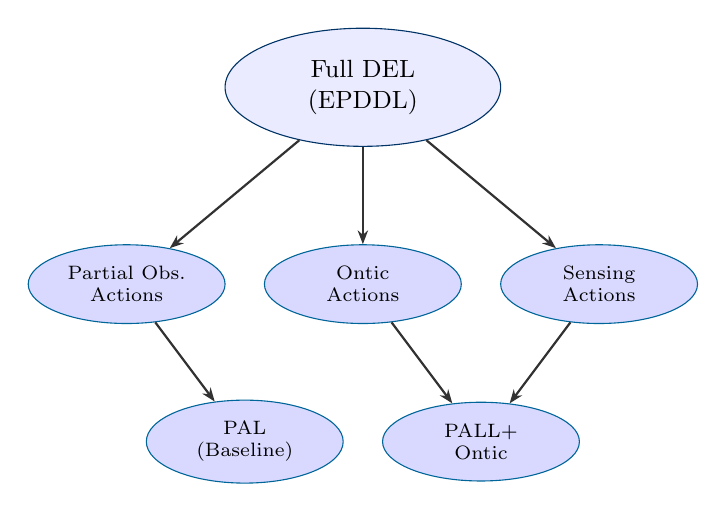
\begin{tikzpicture}[
    frag/.style={ellipse, draw=darkblue, fill=blue!8, minimum width=3.5cm, minimum height=1.5cm, align=center, font=\small},
    subfrag/.style={ellipse, draw=medblue, fill=blue!15, minimum width=2.5cm, minimum height=1cm, align=center, font=\scriptsize},
    arr/.style={-{Stealth[length=5pt]}, thick, darkgray}
]
\node[frag] (del) at (0,0) {Full DEL\\(EPDDL)};
\node[subfrag] (po) at (-3, -2.5) {Partial Obs.\\Actions};
\node[subfrag] (ontic) at (0, -2.5) {Ontic\\Actions};
\node[subfrag] (sensing) at (3, -2.5) {Sensing\\Actions};
\node[subfrag] (pal) at (-1.5, -4.5) {PAL\\(Baseline)};
\node[subfrag] (pall) at (1.5, -4.5) {PALL+\\Ontic};

\draw[arr] (del) -- (po);
\draw[arr] (del) -- (ontic);
\draw[arr] (del) -- (sensing);
\draw[arr] (po) -- (pal);
\draw[arr] (ontic) -- (pall);
\draw[arr] (sensing) -- (pall);
\end{tikzpicture}
\caption{Hierarchy of DEL fragments expressible through EPDDL action type libraries. The baseline (PAL) fragment supports only public announcements. Richer fragments add ontic actions, partial observability, and sensing.}
\label{fig:delfragments}
\end{figure}

\newpage
\section{Integration: Toward a DEL-Based Planning System for ROS2}
\label{sec:integration}

\subsection{Conceptual Architecture}

The integration of DEL-based epistemic planning with a ROS2 multi-robot system requires bridging three conceptual gaps: the gap between the physical robot state and the epistemic state representation, the gap between EPDDL action schemas and ROS2 action server implementations, and the gap between the planner's output (a sequence of abstract epistemic actions) and the robot's execution infrastructure (ROS2 nodes, behavior trees, Nav2, MoveIt2).

We propose a conceptual architecture organized around four principal components:

\textbf{1. Epistemic World Model Manager.} This component maintains the global epistemic state $(M, W_d)$ for the fleet. It receives perception events from individual robots (sensor readings, object detections, communication logs), and updates the Kripke model accordingly---adding or removing worlds, updating labels, and modifying accessibility relations. The update mechanism must implement the product update semantics of DEL, or a suitable approximation for computational tractability.

\textbf{2. EPDDL Planner Interface.} This component translates the current epistemic state into an EPDDL problem specification and calls an external epistemic planner (e.g., one of the solvers submitted to IPC 2026). It receives the plan---a sequence of abstract epistemic actions---and translates it into a sequence of ROS2 dispatchable goals.

\textbf{3. Epistemic Action Dispatcher.} For each abstract epistemic action in the plan, this component instantiates the corresponding physical robot action (if the action is ontic) or communication action (if the action is purely epistemic), and dispatches it to the appropriate ROS2 action server. It also applies the product update to the epistemic model upon action completion, reflecting the new epistemic state.

\textbf{4. Robot Action Servers.} These are the standard ROS2 action server implementations (navigation, manipulation, sensing, communication) that execute the low-level robot behaviors corresponding to EPDDL event instances.

\begin{figure}[H]
\centering
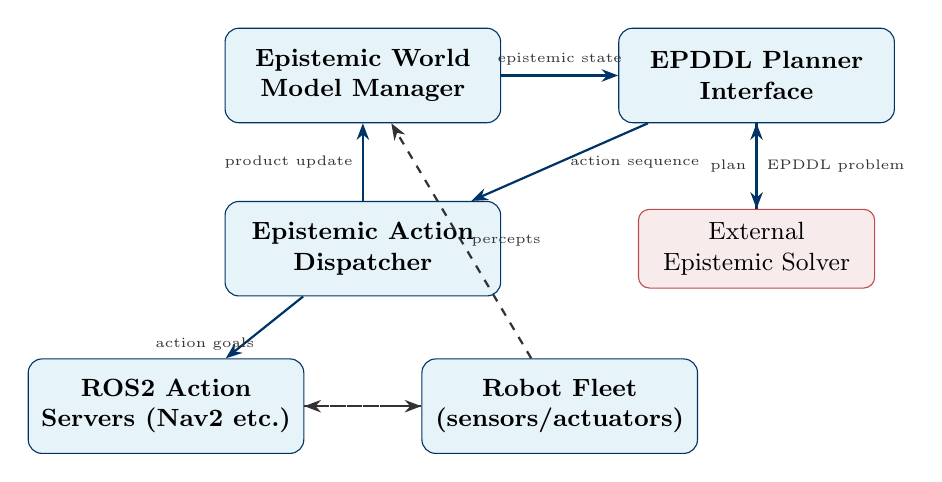
\begin{tikzpicture}[
    comp/.style={rectangle, draw=darkblue, fill=lightblue!30, rounded corners=5pt, minimum width=3.5cm, minimum height=1.2cm, font=\small\bfseries, align=center},
    ext/.style={rectangle, draw=codered!70, fill=codered!8, rounded corners=4pt, minimum width=3cm, minimum height=1cm, font=\small, align=center},
    arr/.style={-{Stealth[length=6pt]}, thick, darkblue},
    darr/.style={-{Stealth[length=6pt]}, thick, darkgray, dashed},
    lbl/.style={font=\tiny, darkgray}
]

\node[comp] (ewm) at (0, 0) {Epistemic World\\Model Manager};
\node[comp] (epi) at (5, 0) {EPDDL Planner\\Interface};
\node[ext] (solver) at (5, -2.2) {External\\Epistemic Solver};
\node[comp] (ead) at (0, -2.2) {Epistemic Action\\Dispatcher};
\node[comp] (ros2) at (-2.5, -4.2) {ROS2 Action\\Servers (Nav2 etc.)};
\node[comp] (robots) at (2.5, -4.2) {Robot Fleet\\(sensors/actuators)};

\draw[arr] (ewm) -- (epi) node[midway, above, lbl]{epistemic state};
\draw[arr] (epi) -- (solver) node[midway, right, lbl]{EPDDL problem};
\draw[arr] (solver) -- (epi) node[midway, left, lbl]{plan};
\draw[arr] (epi) -- (ead) node[midway, right, lbl]{action sequence};
\draw[arr] (ead) -- (ewm) node[midway, left, lbl]{product update};
\draw[arr] (ead) -- (ros2) node[midway, below left, lbl]{action goals};
\draw[darr] (robots) -- (ewm) node[midway, right, lbl]{percepts};
\draw[darr] (ros2) -- (robots);
\draw[darr] (robots) -- (ros2);
\end{tikzpicture}
\caption{Proposed conceptual architecture for a DEL-based epistemic planning system integrated with ROS2. The Epistemic World Model Manager maintains the Kripke model, the EPDDL Planner Interface calls an external solver, and the Epistemic Action Dispatcher bridges the abstract plan to ROS2 action servers.}
\label{fig:integration}
\end{figure}

\subsection{State Space and Computational Challenges}

The most significant computational challenge in implementing this architecture is the size and complexity of the epistemic state space. The number of possible worlds in a Kripke model can grow exponentially with the number of propositions and agents, making both state maintenance and planning intractable for large problems. Several approximation strategies have been explored in the literature:

\textit{Bounded world representations} limit the number of possible worlds to a manageable subset, applying heuristics to prune worlds that are considered unlikely given recent observations. \textit{Belief space planning} maintains probability distributions over worlds (as in POMDPs) rather than possibility sets, enabling more principled approximation at the cost of losing the sharp epistemic semantics. \textit{Compiled classical planning approaches}~\cite{muise2015planning} transform epistemic planning problems into classical planning problems by encoding the epistemic state as additional propositional atoms, enabling the use of efficient classical planners at the cost of expressivity.

\subsection{Perception-to-Epistemic-State Translation}

A critical engineering challenge is the translation of robot sensor data into updates on the Kripke model. A robot's observation---a camera image, a lidar scan, a tactile reading---is a physical signal that must be interpreted as an epistemic event: ``robot $R_1$ now knows whether corridor $c_3$ is blocked.'' This translation requires a perception pipeline that produces discrete, high-level symbolic assertions from raw sensor data, and then models those assertions as epistemic events applied via the product update.

In the ROS2 context, this pipeline would typically consist of a perception node (producing labeled object detections or map observations), a semantic interpretation layer (translating detections into PDDL-compatible ground atoms), and an epistemic update module (applying the product update to the Kripke model maintained by the World Model Manager).

\subsection{Communication Actions as Epistemic Events}

In a multi-robot system, inter-robot communication is itself an epistemic event: when robot $R_1$ broadcasts its observation that corridor $c_3$ is blocked, this constitutes a public announcement of $\Box_{R_1}\mathrm{corridorBlocked}(c_3)$, and the epistemic state of the fleet changes according to the DEL product update. This is a powerful and natural modelling capability that DEL provides: communication is not an ad hoc side channel but a first-class epistemic action with formally defined effects on the knowledge state of all agents.

In the proposed architecture, the Epistemic Action Dispatcher would implement communication actions as ROS2 topic publications or service calls, and would simultaneously apply the corresponding product update to the World Model Manager.

\subsection{Open Research Questions}

The integration outlined above raises a number of open research questions that define the scope of the planned research agenda:

\textbf{Tractable epistemic state representations.} What representations of the Kripke model are expressive enough to support EPDDL-level reasoning yet compact enough to be maintained in real time for multi-robot fleets? Are factored Kripke models or compiled representations sufficient for the target class of problems?

\textbf{Online epistemic planning.} Classical task planners in ROS2 are invoked reactively when the world state changes. Epistemic planners must similarly support online replanning when new observations arrive. What are the performance characteristics of available epistemic planners (e.g., EFP, mGPT, MCEPlan) in online settings?

\textbf{EPDDL-to-ROS2 toolchain.} How should the \texttt{plank} toolkit be integrated with the ROS2 build and runtime systems? Can EPDDL domain and problem files be automatically generated from ROS2 system descriptions and runtime state?

\textbf{Epistemic goal specification.} How should a human operator or a fleet management system specify epistemic goals in a ROS2 context? What user interface abstractions are appropriate for specifying goals such as ``ensure that all robots know whether the target room is occupied''?

\textbf{Failure handling.} How should epistemic plan failures be handled? If an action's precondition fails, the epistemic state must be updated accordingly and a new plan generated. What recovery strategies are appropriate for epistemic plan failures in a ROS2 runtime?


\newpage
\bibliographystyle{plain}
\begin{thebibliography}{99}

\bibitem{macenski2022robot}
Macenski, S., Foote, T., Gerkey, B., Lalancette, C., \& Woodall, W. (2022).
\textit{Robot Operating System 2: Design, architecture, and uses in the wild}.
Science Robotics, 7(66).

\bibitem{martin2021plansys2}
Mart\'in, F., Mateos, J., Vargas, F., Moreno, R., Fernandez-Rodr\'iguez, J.~C., \& Ginesi, A. (2021).
\textit{PlanSys2: A Planning System Framework for ROS2}.
In Proceedings of the IEEE/RSJ International Conference on Intelligent Robots and Systems (IROS).

\bibitem{baltag1998logic}
Baltag, A., Moss, L.~S., \& Solecki, S. (1998).
\textit{The Logic of Public Announcements, Common Knowledge and Private Suspicions}.
In Proceedings of the 7th Conference on Theoretical Aspects of Rationality and Knowledge (TARK-98).

\bibitem{vanditmarsch2007}
van Ditmarsch, H., van der Hoek, W., \& Kooi, B.~P. (2007).
\textit{Dynamic Epistemic Logic}. Volume 337.
Springer Netherlands.

\bibitem{burigana2026epddl}
Burigana, A., \& Fabiano, F. (2026).
\textit{The Epistemic Planning Domain Definition Language: Official Guideline}.
Official Guideline Reference for the Epistemic Planning Track at IPC-26.

\bibitem{bolander2011epistemic}
Bolander, T., \& Andersen, M.~B. (2011).
\textit{Epistemic Planning for Single- and Multi-Agent Systems}.
Journal of Applied Non-Classical Logics, 21(1), 9--34.

\bibitem{coles2010forward}
Coles, A., Coles, A., Fox, M., \& Long, D. (2010).
\textit{Forward-Chaining Partial-Order Planning}.
In Proceedings of ICAPS.

\bibitem{faconti2018behaviortree}
Faconti, D., \& Colledanchise, M. (2018).
\textit{BehaviorTree.CPP: A Behavior Tree Library for C++}.
Available: \url{https://www.behaviortree.dev}.

\bibitem{openrmf2021}
Open Robotics (2021).
\textit{Open-RMF: Open Robotics Middleware Framework}.
Available: \url{https://www.open-rmf.org}.

\bibitem{muise2015planning}
Muise, C., Belle, V., Felli, P., McIlraith, S.~A., Miller, T., Pearce, A.~R., \& Sonenberg, L. (2015).
\textit{Planning Over Multi-Agent Epistemic States: A Classical Planning Approach}.
In Proceedings of AAAI 2015.

\bibitem{son2014finitary}
Son, T.~C., Pontelli, E., Baral, C., \& Gelfond, G. (2014).
\textit{Finitary S5-Theories}.
In Proceedings of JELIA 2014. Lecture Notes in Computer Science, vol. 8761, Springer.

\bibitem{kominis2015beliefs}
Kominis, F., \& Geffner, H. (2015).
\textit{Beliefs in Multiagent Planning: From One Agent to Many}.
In Proceedings of ICAPS 2015.

\bibitem{hintikka1962knowledge}
Hintikka, J. (1962).
\textit{Knowledge and Belief: An Introduction to the Logic of the Two Notions}.
Cornell University Press.

\bibitem{ghallab2004automated}
Ghallab, M., Nau, D.~S., \& Traverso, P. (2004).
\textit{Automated Planning: Theory and Practice}.
Elsevier.

\end{thebibliography}

\end{document}